\subsection{Ingest data directly with BigQuery}
\subsubsection{Prerequisites and Setup}
\begin{itemize}
    \item Google Cloud Storage (GCS) Bucket: This is where your CSV file is stored. Ensure the file is in a publicly accessible location or that you have the necessary permissions to access it.
\item BigQuery Dataset: Your target dataset in BigQuery should already be created. If not, create one by navigating to the BigQuery console, clicking on your project, and selecting Create Dataset. You will be prompted to specify a dataset ID, data location, and any expiration date or encryption preferences.
\end{itemize}
\subsubsection{Load data with BigQuery}
Big Query support loading CSV data from Cloud Storage in multiple options such as SQL, Console and more. In this project, our team choose to use bq command-line tool of Big Query to load data into table in Big Query. The reason of this choice lies mainly in the fact that Big Query supports auto detection for CSV file, which ,as the name suggests, automatically detect the schema and data type. Auto detection leads to the conflict between detected data type and our desired schema or not so well-formatted data. Unlike SQL (main tools we use for ingest data with BigQuery), bq command-line tool supports option for turning off auto detection. The bq command we use is as below:
\begin{lstlisting}
bq  load --replace --source_format=CSV --autodetect=false --field_delimiter='|' --skip_leading_rows=1  --max_bad_records=1000 --quote "" bigquery_direct.saleheader_raw_loading  'gs://retailer-raw-ingest-data/SalesHeaderFCT_inc_20240929.txt' 
\end{lstlisting}
The options are listed as:
\begin{itemize}
    \item --replace: To erase any existing data and schema when new data is loaded
    \item --autodetect=false: Turn off schema auto detection
    \item --field\_delimiter='|' : Specifies the character that marks the boundary between columns in the data
    \item  --skip\_leading\_rows=1: Skip header row
    \item --max\_bad\_records=1000: Skip bad record (such as row missing columns in CSV data)
    \item --quote "": Specify that there is no quote character to surround fields in CSV data
\end{itemize}
\subsubsection{From Cloud Storage to the main table in BigQuery}
Although we can directly load data into table in BigQuery, the format of some of our data do not match with one default format in BigQuery, especially with DATE and DATETIME data type, moreover some columns ' majority values are NULL, hence our team decide to load in temporary tables before transform it into correct data format in main tables with column having small proportion of NULL.\\
In this scope of project, we call the second tables used for directly loaded data temporary tables to emphasize that they only hold data for a short time. However the tables are just normal tables, not temporary tables BigQuery provides. The temporary tables have all the columns in CSV files, with data type all set to string for the ease of load every data format. 
\begin{figure}[!h]
    \centering
    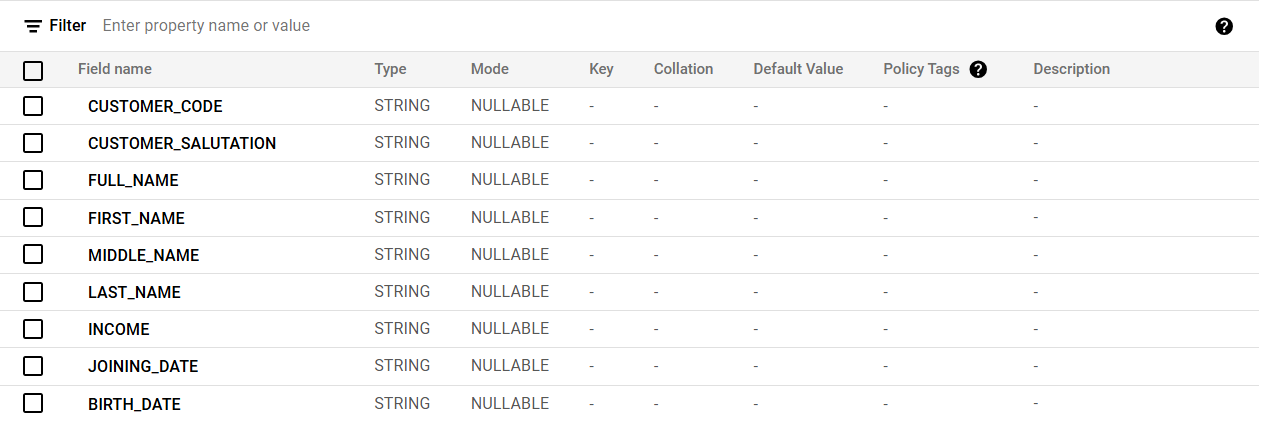
\includegraphics[width=0.75\linewidth]{images/temporary_product_table.png}
    \caption{Temporary table for product record }
\end{figure}

The process of loading CSV file from Cloud Storage to temporary tables in BigQuery took approximately 25 seconds for 140MB data as below. 
\begin{figure}[htp]
    \centering
    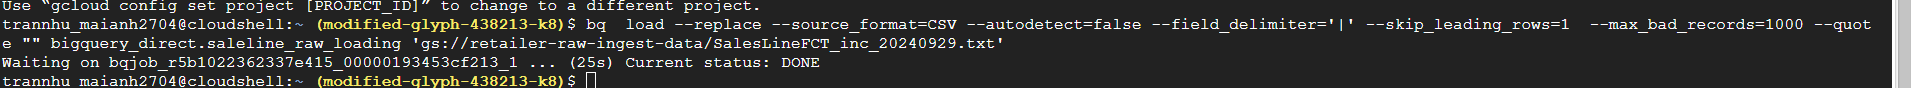
\includegraphics[width=0.75\linewidth]{images/timeproccess.png}
   \caption{SaleLine data file is around 140MB}
\end{figure}
\\After loading into temporary tables, we update all empty string with NULL VALUE. This step is optional and can be replaced by using safe\_cast() which replaces runtime errors (invalid format) with NULL. Hence this step helps decide which columns to keep by reporting the ration of NULL values over number of records. 
\begin{figure}[htp]
    \centering
    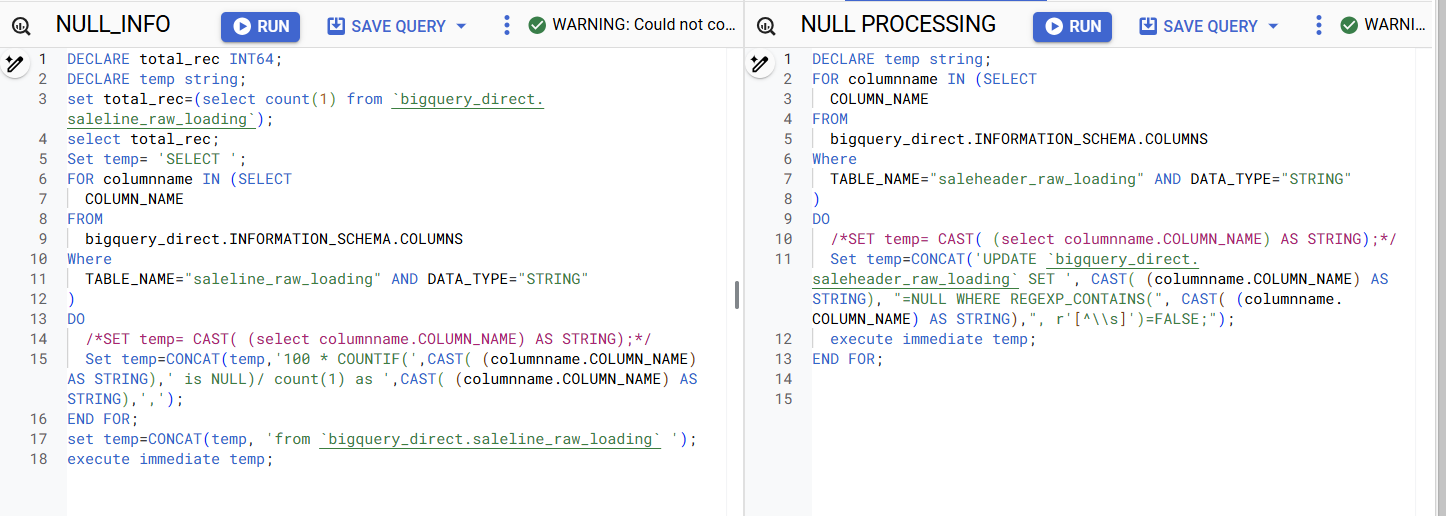
\includegraphics[width=0.75\linewidth]{images/NULL_PROC.png}
\end{figure}
\\The process of updating NULL value took approximately 1 min 10 seconds for 140MB data as below. 
\clearpage
\begin{figure}[htp]
    \centering
    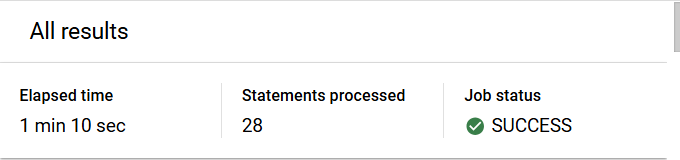
\includegraphics[width=0.75\linewidth]{images/NULLtime.png}
\end{figure}
When inserting from temporary table into main table, we cast data into desired data type. For some special data type, we need to modify a little bit. For DATETIME data type, we cast on the sub string of data to remove the excessive fractional parts. For GEOGRAPHY data type, we change a string into ST\_GEOGPOINT for future work as below.  Furthermore, we can set some attribute for columns when inserting by using WHERE clause, such as forcing a column with unique values or a column only contains value in another table like a FOREIGN KEY. After inserting, we truncate the temporary tables to reduce the storage we used.
\begin{figure}[htp]
    \centering
    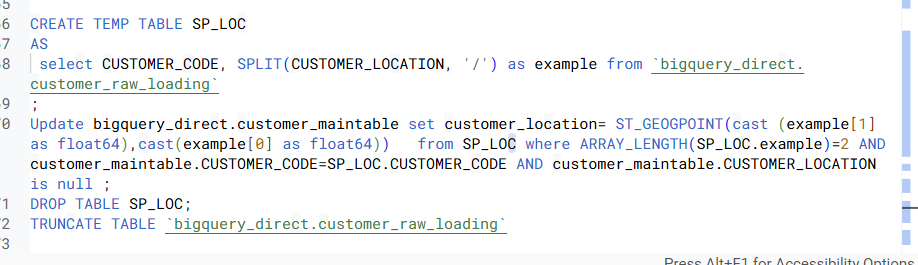
\includegraphics[width=0.75\linewidth]{images/process data.png}
    \caption{Process GEOGRAPHY data type}
\end{figure}
\begin{figure}[htp]
    \centering
    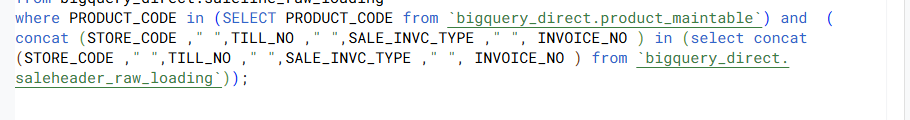
\includegraphics[width=0.75\linewidth]{images/foreign key.png}
    \caption{Force SaleLine Table to have matching sale header and contains only registered products}
    \label{fig:enter-label}
\end{figure}

The process of inserting took approximately 10 seconds for 140MB data as below. 
\begin{figure}[!htp]
    \centering
    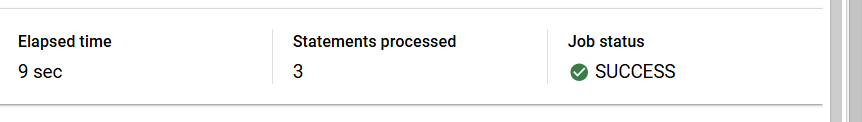
\includegraphics[width=0.75\linewidth]{images/inserttime.png}
\end{figure}
\\
\subsubsection{Result}
    To sum up, the process from Cloud storage into BigQuery took approximately 1 minute 45 seconds for 140MB data, with the majority goes to process the NULL values. The quality of the final data was ensured by using WHERE clause when inserting into main table and transformation process on raw data. The final data therefore is ensured to be accurate  and reliable.
    \\\\
    The main challenges encountered during the data ingestion process is handling data format and NULL value to reduce the veracity of Big Data. By using appropriate SQL statement to validate data before append them into our main table, we lower the veracity by remove those entries with noise or abnormal value. Lessons learned from veracity challenges include the importance of data Knowledge retrieved from testing and the need for input validation before merging the data into the main table.
